%!TEX root = main.tex
%%%%%%%%%%%%%%%%%%%%%%%%%%%%%%%%%%%%%%%%%%%%%%%%%%%%%%%%%%%%%%%%%%%%%%%%%%%%%%%%%%%%%%%%%%%%%%%%%%%%%%
%
%   Filename    : appendix_A.tex 
%
%   Description : This file is one of the appendices. 
%                 
%%%%%%%%%%%%%%%%%%%%%%%%%%%%%%%%%%%%%%%%%%%%%%%%%%%%%%%%%%%%%%%%%%%%%%%%%%%%%%%%%%%%%%%%%%%%%%%%%%%%%%

\chapter{Research Ethics Forms}
\label{sec:appendixa}

\chapter{Turnitin Similarity Report}
\label{sec:appendixb}

\chapter{Record of Contribution}

% \chapter{Data Collection Artifacts}
% \label{sec:appendixc}

\begin{comment}
\chapter{Design Artifacts}
\label{sec:appendixd}

\section{Affinity Diagram}
\newpage
\end{comment}

\chapter{Literature Map}
  \label{sec:appendixe}


  \begin{sidewaysfigure}[h]
      %\centering
    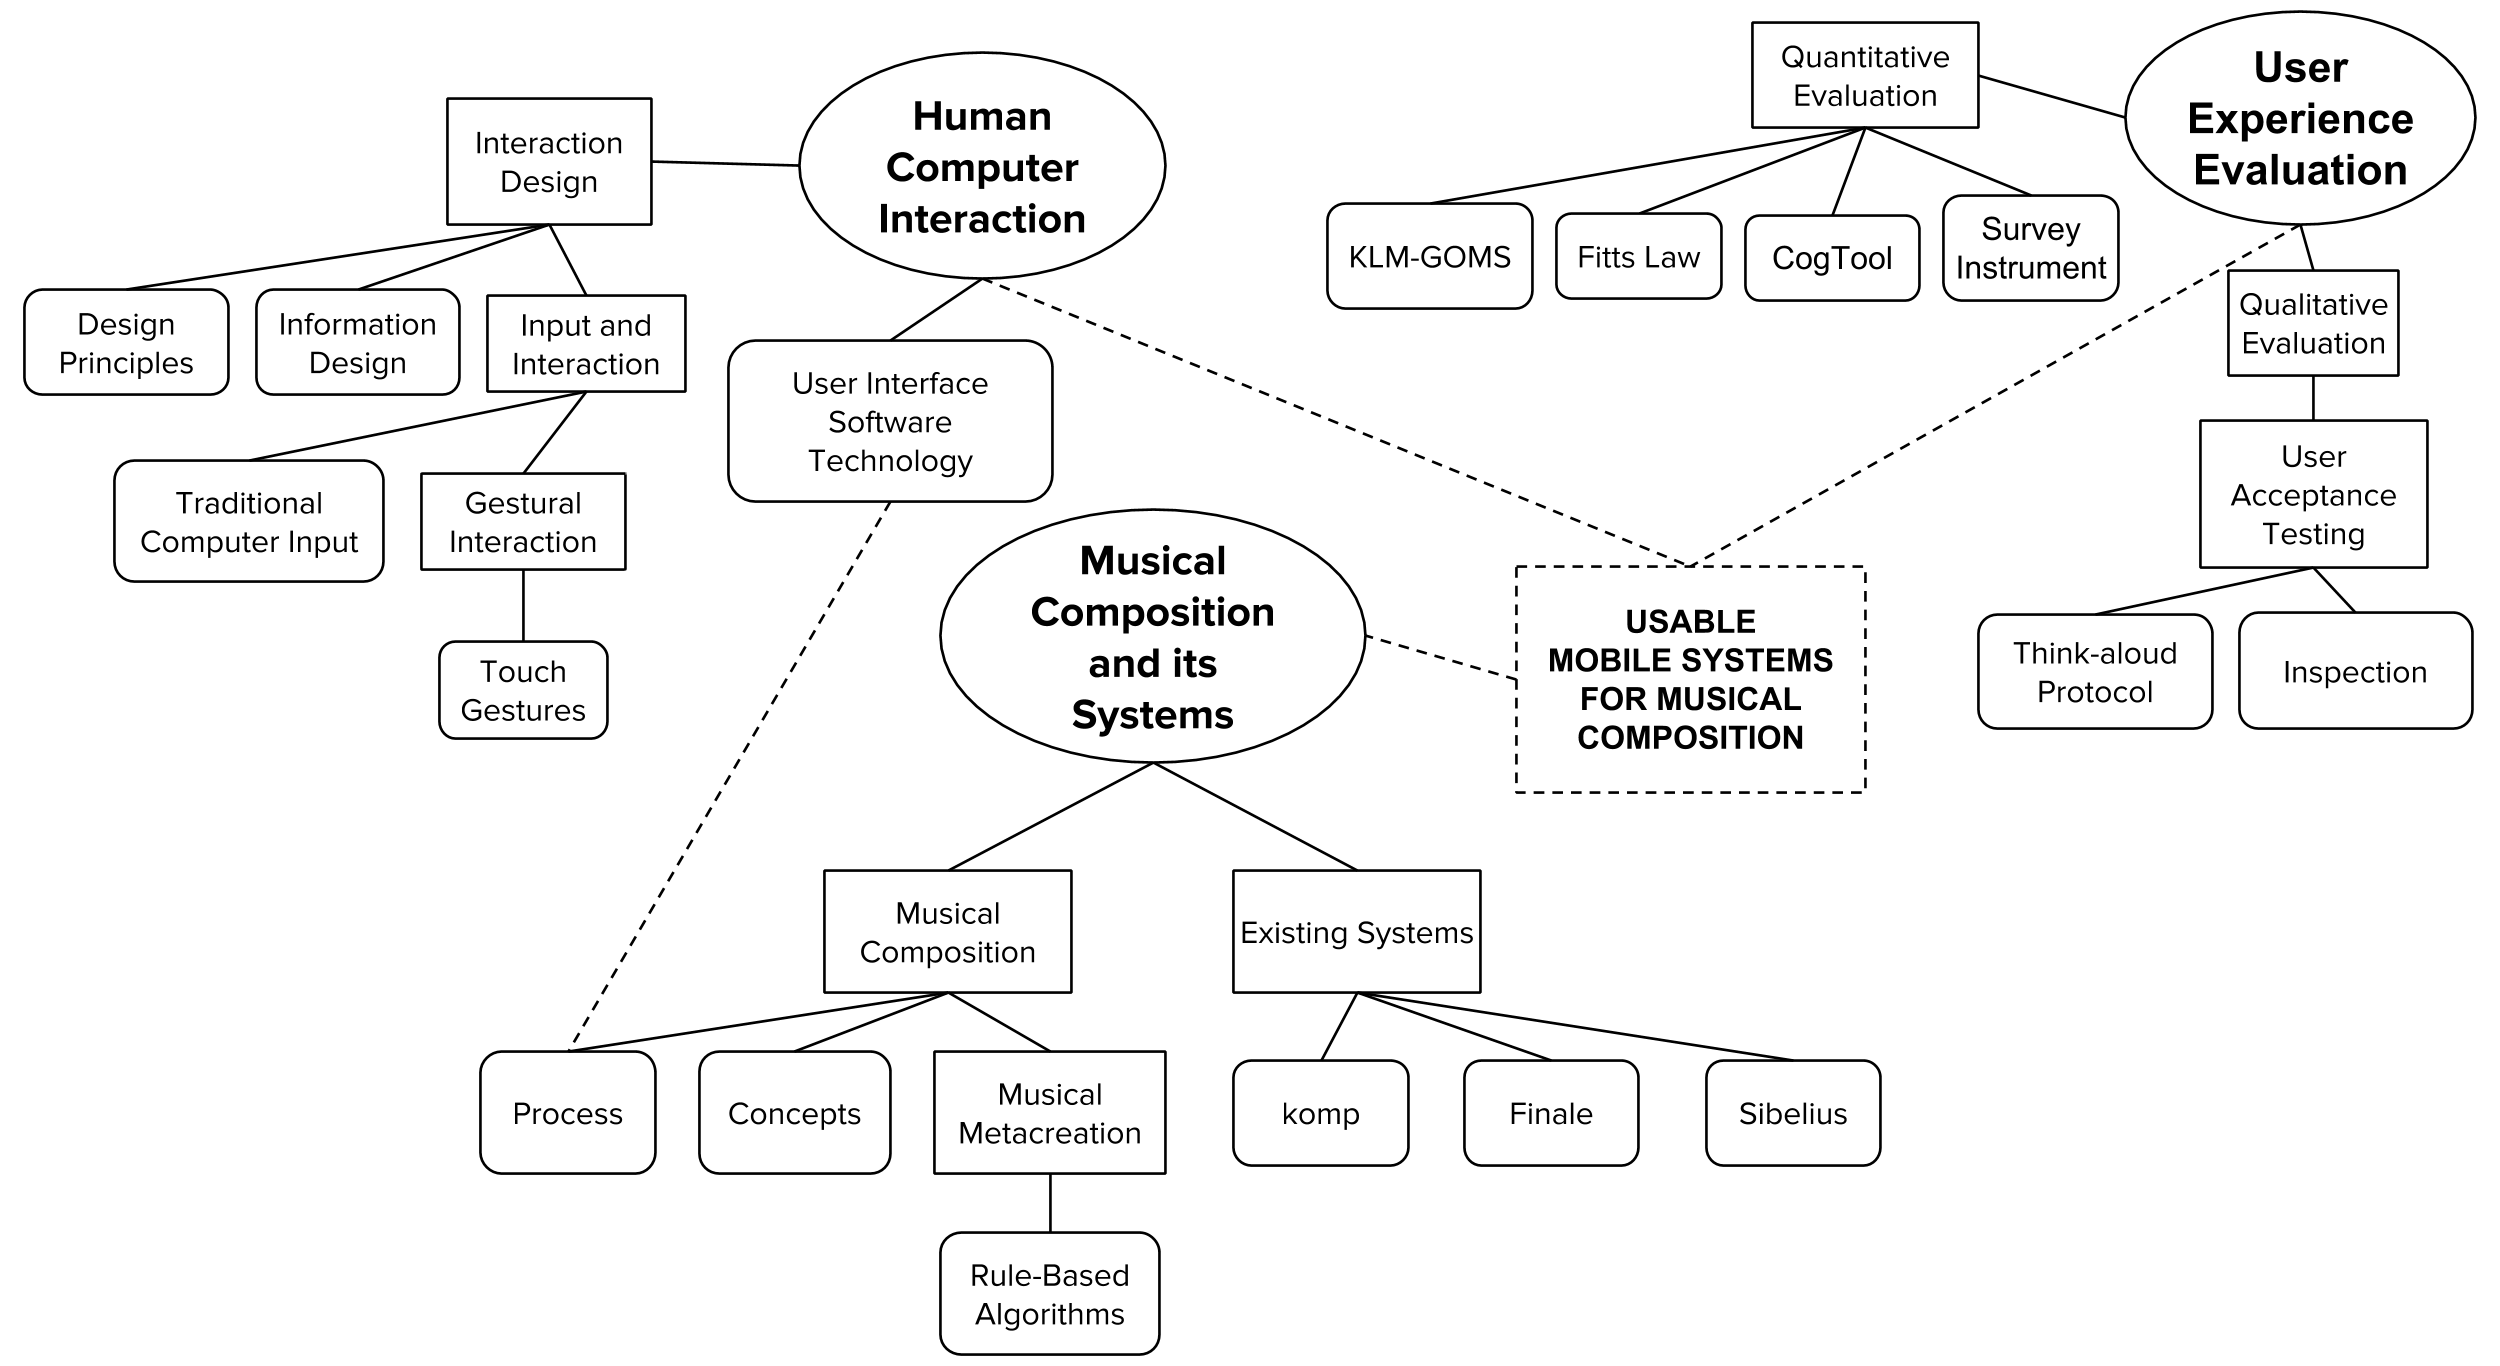
\includegraphics[scale=0.26]{literature_map}
      \caption{Literature map.}
      \label{fig:literature-map}
  \end{sidewaysfigure}

\chapter{User Personas}
\label{sec:user-personas}

  \begin{comment}
  \begin{wrapfigure}{l}{0.5\textwidth}

    \begin{center}
      
\includegraphics[width=0.48\textwidth]{mary_persona}
    \end{center}
  \end{wrapfigure}
  \end{comment}

  \subsection{Mary: The Amateur}

  \begin{itemize}
  \item 18 years old
  \item Started composing as a hobby when she was 16 years old
  \item 2nd Year undergraduate student
  \item Currently taking up a Bachelor in Music degree program
  \item Passing grades during her 1st Year
  \end{itemize}

  "Its such a hassle to write notes on music sheets. Its hard to keep track which are the drafts."

  "I haven't found any app like Finale in the app store."

  Mary lives in a dorm with 3 other people and has her own laptop and tablet. She uses both of these devices to do her work in any place.

  Mary mostly uses music sheets when she needs to compose music for assignments. She usually uses her laptop for research and the tablet as a substitute when she doesn't feel like bringing her laptop.

  Mary has passing marks in her courses. She experiences difficulty getting high grades because she has a hard time looking for inspiration and ideas. She also easily gets tired writing, revising, and finalizing her compositions on paper.

  She is knowledgeable in using Sibelius on her laptop and has started to learn Finale due to her professors urging her to use it. She appreciates how these kinds of applications reduce the steps in some repetitive or tedious processes in composing music.

  \begin{comment}
  \begin{wrapfigure}{l}{0.5\textwidth}
    \begin{center}
    
      
\includegraphics[width=0.48\textwidth]{warren_persona}
    \end{center}
  \end{wrapfigure}
  \end{comment}

  \subsection{Warren: The Experienced}

  \begin{itemize}
  \item 34 years old
  \item 10 years of composing music professionally
  \item Music teacher in a high school
  \item Loves classical music
  \item Music fundamentalist
  \item Wants his students to be more engaged in music and appreciate the art form
  \item Faculty for 5 years
  \end{itemize}

  "Music is a way to truly express yourself"

  "I want to share my passion in music to my pupils"

  Warren is currently a faculty member of a private high school that pays him enough that he can make a living and support his family.

  Warren has been teaching for 5 years. He has been involved in organizing the curriculum in the school. He has always believed that music as an art form is timeless and should be learned by everyone.

  He wants his students to appreciate music as much as he does. He shares the works of Beethoven and Mozart, which are his favorites, to his class.

  % He wants his students to appreciate music since years of hard work from various authors like Beethoven and Mozart have devoted their whole lives to the art. 

  He often observes students using their mobile devices in school. During class, he's made it clear that the usage of cellphones is restricted. However, he understands the potential of these mobile devices as tools for musical composition.

  % He often observes students being too distracted with their devices in school. During class, he's made it clear that the usage of cellphones is restricted. Though, he can see the usefulness of the technology for research and some classes in his school has integrated e-learning.

  He is experienced in using Finale but still uses music sheets during occasions where he cannot use his laptop or is still sketching. He has been wondering whether there is a viable mobile alternative to using music sheets.

  % He's been wondering if these technologies can be used for teaching music but he's on the fence about it because students might not experience music fully.


  \begin{comment}
  \begin{wrapfigure}{l}{0.5\textwidth}
    \begin{center}
      
\includegraphics[width=0.48\textwidth]{winston_persona}
    \end{center}
  \end{wrapfigure}
  \end{comment}

  \subsection{Winston: The Veteran}

  \begin{itemize}
  \item 62 Years Old
  \item 40 years of experience in composing music professionally
  \item Composes music for different companies and artists
  \item Mentors up and coming composers
  %\item Active in international conferences about the field of Music
  \item Married for 35 years
  \item Has experienced the numerous shifts of popularity between music genres
  \end{itemize}

  "Music has always been a part of everyone's lives" 

  "I wonder whats next the next big thing that can change music" 

  Warren always reads on music-related news and enjoys doing research on topics that concern music. He writes his findings and his thoughts on his blog. He has lived through several shifts in mainstream music and has studied the change agent in every shift. 

  He has been able to adjust and make a living from these hobbies. He has always been able to make music that matched what was popular at the time. He fully accepts that music changes for every new generation of artists and composers.

  He is waiting for the next big thing that can happen for music, always prepared to make the needed adjustments to stay in the game. He is no stranger to using technology like Finale or Sibelius to compose his pieces.

\begin{comment}
\chapter{Resource Persons}
\label{sec:appendixf}

\newcommand{\resperson}[4]{\textbf{#1} \\ #2 \\ #3 \\ \url{#4}\vspace{0.5em}\\}

\resperson{Mr. Jordan Aiko Deja}{Adviser}{College of Computer Studies\\De La Salle University-Manila}{jordan.deja@dlsu.edu.ph}
\\
\resperson{Dr. Rafael Cabredo}{Chair, Software Technology Department}{College of Computer Studies\\De La Salle University-Manila}{rafael.cabredo@dlsu.edu.ph}

\end{comment}

\chapter{User Stories}
  The user stories of the system will be focused on the main functions of the application and will highlight each specific need that the user has for the system. These user stories came from identified user needs, representing the tasks that they need to perform on musical composition applications. These are created with the context that the system will run on a mobile platform with the mode of interaction mainly being touch gestures. 

  \begin{itemize}
    \item As a user, I want to be able to create a blank composition, so that I can start my work
    \item As a user, I want to be able to name my composition, so that I can differentiate it from my other compositions
    \item As a user, I want to be able to save my composition, so that I can come back to it later
    \item As a user, I want to be able to view all my saved compositions in a list, so that I can keep track of everything
    \item As a user, I want to be able to open a saved composition so that I can perform more actions on it
    \item As a user, I want to be able export my composition in a format that I can open in the composition application I use on my laptop
    \item As a user, I want to be able to delete a composition, so I can discard compositions I do not work on anymore
    \item As a user, I want to be able to add a chord progression in my composition, so that I do not need to individually add notes that belong to a progression
    \item As a user, I want to be able to place a note in my composition, so that I can create my composition
    \item As a user, I want to be able to select a single note, so that I can perform actions on it
    \item As a user, I want to be able to change the pitch class of a note in my composition, so that I can make adjustments to my composition
    \item As a user, I want to be able to change the type of a note in my composition, so that I can make the sound longer or shorter
    \item As a user, I want to be able to erase a note in my composition, so that I can make space for other notes in my composition
    \item As a user, I want to be able to highlight a group of notes in my composition, so that I can perform actions on the group
    \item As a user, I want to be able to erase a highlighted group of notes in my composition, so that I can make space faster for other notes I'd like to place in my composition
    \item As a user, I want to be able to place a rest in my composition, so I can have pauses in my composition
    \item As a user, I want to be able to select a rest, so that I can perform actions on that rest
    \item As a user, I want to be able to change the type of rest, so that I can change the length of pauses
    \item As a user, I want to be able to highlight a group of rests, so that I can perform actions on the group of rests
    \item As a user, I want to be able to erase a rest in my composition, so that I can make space for other rests or notes
    \item As a user, I want to be able to change a rest in my composition, so that I can make adjustments to my composition
    %\item As a user, I want to be able to move the position of a note in my composition, so that I can move that note to a better position
    %\item As a user, I want to be able to move the position of a highlighted group of notes in my composition, so that I can reposition multiple notes at a time to a better position
    \item As a user, I want to be able to hear the sound of the note I just added, so that I know I've added the correct sounding note
    \item As a user, I want to be able to listen to a highlighted section of my composition, so that I can hear just a segment of my piece
    \item As a user, I want to be able to listen to my whole composition, so that I can hear it as a whole
    \item As a user, I want to be able to perform a swipe gesture that will generate a succession of notes based on the orientation of my gesture and my current composition because I'm interested in knowing what series of notes match my current composition
    \item As a user, I want to be able to manipulate the generated series of notes, because the generated series of notes just needs a little bit more adjustments before I accept it into my composition
    \item As a user, I want to be able to discard the series of notes generated by the application after a swipe gesture, so I do not have to delete them one by one
    \item As a user, I want to be able to confirm the addition of the series of notes given by the application after a swipe gesture, so I can create my composition quickly
    \item As a user I want to be able to undo an action or a series of actions, so that I can undo an unintended action or series of unintended actions quicker
    \item As a user I want to be able to redo an action or a series of actions, so that I can redo an intended action or a series of intended actions quicker
    \item As a user, I want to be able to reposition the menu because I want to place it where it is not an obstacle for me while composing
    \item As a user, I want to be able to set the time signature of my composition
    \item As a user, I want to be able to see the details of a single note, so that I can know the specifications of the note
    \item As a user, I want to be able to see the details of a selected group of notes, so that I can know the specification of the selected group of notes
    \item As a user, I want to be able to see the details of the generated series of notes like the pitch and type so that I can know what notes the system has generated after a gesture
    \item As a user, I want to be able to set the clef of my composition
    \item As a user, I want to be able to set the key signature of my composition
    \item As a user, I want to be able to set the time signature of my composition
    \item As a user, I want to be able to copy a highlighted group of notes and/or rests, so that I can copy a recurring segment in my composition
    \item As a user, I want to be able to cut a highlighted group of notes and/or rests, so that I can copy a segment of my composition while at the same time making space for more notes
    \item As a user, I want to be able to paste the copied or cut group of notes and/or rests onto my composition, so that I do not need to add a recurring segment in my composition manually all the time
    %\item As a user, I want to be able to move the position of a rest, so that I can move that rest to a better position
    %\item As a user, I want to be able to move the position of a selected group of rests, so that I can move multiple rests at a time to a better position
    \item As a user, I want to be able to add accidentals to my notes, so that I can control the pitch of my notes
    \item As a user, I want to be able to transpose a highlighted group of notes, so that I do not need to individually change the pitch of each note
    \item As a user, I want to be able to perform retrograde inversion on a single note, so that I do not have to move it manually to invert it
    \item As a user, I want to be able to perform retrograde inversion on a group of notes, so that I do not need to invert each note individually
  \end{itemize}

\chapter{Use Cases}

  This chapter defines the several actions the users can perform within the system. These use cases were derived from the needs of the composers and the functions of Flow. The design of each use case will be based on fully dressed use cases with precision level 2 found in the book of \cite{alistair2001writing}. The headers in each use case will be: trigger, primary actor, supporting actors, preconditions, minimal guarantees, success guarantees, and process steps.

  \textbf{Trigger} \\
  The main situation or goal that the use case will be revolving around. 

  \textbf{Primary Actor} \\
  The main entity that will be performing or influencing situation or goal directly.

  \textbf{Supporting Actors} \\
  Additional entities that will be indirectly or directly influenced by the outcome of the situation. These entities can also be influencing the decision making or performance of the primary actor.

  \textbf{Preconditions} \\
  These conditions need to be followed before the process steps can be performed.

  \textbf{Process Steps} \\
  Each step will be performed by the primary actor to accomplish the goal.

  \textbf{Minimal Guarantees} \\
  Outcome or result that will occur in case a goal is not fully accomplished.

  \textbf{Success Guarantees} \\
  Outcome or result that occurs when a goal is fully accomplished.

  %Trigger
  %Primary Actor
  %Supporting Actors
  %Precondition
  %Process Steps
  %Minimal Guarantees
  %Success Guarantees


  %%Layout needs to be fixed

  %Sprint 1
  \subsubsection{Use Case 1: Add a Single Note}

  \LTXtable{\textwidth}{longtables/use_case_1_lt}

  %Sprint 1
  \subsubsection{Use Case 2: Change a Single Note}

  \LTXtable{\textwidth}{longtables/use_case_2_lt}

  %Sprint 1
  \subsubsection{Use Case 3: Delete a Single Note through the Side Menu}

  \LTXtable{\textwidth}{longtables/use_case_3_lt}

  \subsubsection{Use Case 4: Delete a Single Note through a Flick Gesture}

  \begin{tabularx}{\textwidth}{|X|X|}
  \hline
  Trigger & 
  The composer needs to delete a note quickly \\
  \hline
  Primary Actor & 
  Composer\\
  \hline
  Supporting Actors & 
  \begin{itemize}
  \item Listener
  \item Instrumentalist
  \item Producer
  \item Flow
  \end{itemize} \\
  \hline
  Precondition & 
  \begin{itemize}
  \item The user has a composition open in Flow 
  \item The deletion of the selected note is valid based on the set musical rules
  \end{itemize} \\
  \hline
  Process Steps & 
  \begin{enumerate}
  \item The user performs a flick gesture on the note to be deleted
  \item Flow removes the selected note from the composition
  \end{enumerate} \\
  \hline
  Minimal Guarantees & 
  \begin{itemize}
    \item A note will be deleted
    \item The side menu will return to being transparent
  \end{itemize} \\
  \hline
  Success Guarantees & 
  \begin{itemize}
    \item The selected note will be deleted
    \item The space occupied by the selected note will be freed
  \end{itemize} \\
  \hline
  \end{tabularx}

  \subsubsection{Use Case 5: Toggle Accidental Marks on Note Addition}

  \LTXtable{\textwidth}{longtables/use_case_5_lt}

  \subsubsection{Use Case 6: Transform a Note to its Dotted Version}

  \LTXtable{\textwidth}{longtables/use_case_6_lt}

  \subsubsection{Use Case 7: Horizontal Swipe Gesture to Generate a Series of Notes}

  \LTXtable{\textwidth}{longtables/use_case_7_lt}

  \subsubsection{Use Case 8: Delete a Highlighted Group of Notes or Rests}

  \LTXtable{\textwidth}{longtables/use_case_8_lt}

  \subsubsection{Use Case 9: Replace a Highlighted Group of Notes or Rests with a Single Note}

  \LTXtable{\textwidth}{longtables/use_case_9_lt}

  \subsubsection{Use Case 10: Replace a Highlighted Group of Notes or Rests with a Single Rest}

  \LTXtable{\textwidth}{longtables/use_case_10_lt}


  \subsubsection{Use Case 11: Single Note Transposition}

  \begin{tabularx}{\textwidth}{|X|X|}
  \hline
  Trigger & 
  The user needs to transpose a note to set its pitch higher \\
  \hline
  Primary Actor & 
  Composer \\
  \hline
  Supporting Actors & 
  \begin{itemize}
  \item Listener
  \item Instrumentalist
  \item Producer
  \item Flow
  \end{itemize} \\
  \hline
  Precondition & 
  \begin{itemize}
  \item The user has a composition open in Flow
  \item The transposition is valid based on the set musical rules
  \end{itemize} \\
  \hline
  Process Steps & 
  \begin{enumerate}
  \item The user performs a two finger swipe gesture upwards on the desired note
  \item Flow increases the pitch of the note
  \end{enumerate} \\
  \hline
  Minimal Guarantees & 
  \begin{itemize}
    \item None
  \end{itemize} \\
  \hline
  Success Guarantees & 
  \begin{itemize}
    \item The desired note will be transposed upwards
  \end{itemize} \\
  \hline
  \end{tabularx}

  \subsubsection{Use Case 12: Multiple Note Transposition}

  \begin{tabularx}{\textwidth}{|X|X|}
  \hline
  Trigger & 
  The user needs to transpose a group of note to set their pitch higher \\
  \hline
  Primary Actor & 
  Composer \\
  \hline
  Supporting Actors & 
  \begin{itemize}
  \item Listener
  \item Instrumentalist
  \item Producer
  \item Flow
  \end{itemize} \\
  \hline
  Precondition & 
  \begin{itemize}
  \item The user has a composition open in Flow
  \item The batch transposition is valid based on the set musical rules
  \end{itemize} \\
  \hline
  Process Steps & 
  \begin{enumerate}
  \item The user highlights a group of notes
  \item The user performs a two finger swipe gesture upwards on the highlighted group of notes
  \item Flow increases the pitch of the highlighted group of notes
  \end{enumerate} \\
  \hline
  Minimal Guarantees & 
  \begin{itemize}
    \item None
  \end{itemize} \\
  \hline
  Success Guarantees & 
  \begin{itemize}
    \item The highlighted group of notes will be transposed upwards
  \end{itemize} \\
  \hline
  \end{tabularx}


  \subsubsection{Use Case 13: Retrograde a Collection of Notes}

  \begin{tabularx}{\textwidth}{|X|X|}
  \hline
  Trigger & 
  The user needs to retrograde a collection of notes \\
  \hline
  Primary Actor & 
  Composer \\
  \hline
  Supporting Actors & 
  \begin{itemize}
  \item Listener
  \item Instrumentalist
  \item Producer
  \item Flow
  \end{itemize} \\
  \hline
  Precondition & 
  \begin{itemize}
  \item The user has a composition open in Flow
  \item The retrograde does not violate the set musical rules
  \end{itemize} \\
  \hline
  Process Steps & 
  \begin{enumerate}
  \item The user highlights a group of notes
  \item The user performs a two finger flick gesture horizontally on top of the collection of notes
  \item Flow retrogrades the collection of notes
  \end{enumerate} \\
  \hline
  Minimal Guarantees & 
  \begin{itemize}
    \item None
  \end{itemize} \\
  \hline
  Success Guarantees & 
  \begin{itemize}
    \item The collection of notes will be retrograded
  \end{itemize} \\
  \hline
  \end{tabularx}

  \subsubsection{Use Case 14: Invert a Collection of Notes}

  \begin{tabularx}{\textwidth}{|X|X|}
  \hline
  Trigger & 
  The user needs to invert a collection of notes \\
  \hline
  Primary Actor & 
  Composer \\
  \hline
  Supporting Actors & 
  \begin{itemize}
  \item Listener
  \item Instrumentalist
  \item Producer
  \item Flow
  \end{itemize} \\
  \hline
  Precondition & 
  \begin{itemize}
  \item The user has a composition open in Flow
  \item The inversion does not violate the set musical rules
  \end{itemize} \\
  \hline
  Process Steps & 
  \begin{enumerate}
  \item The user highlights a group of notes
  \item The user performs a two finger flick gesture vertically on top of the collection of notes
  \item Flow inverts the collection of notes
  \end{enumerate} \\
  \hline
  Minimal Guarantees & 
  \begin{itemize}
    \item None
  \end{itemize} \\
  \hline
  Success Guarantees & 
  \begin{itemize}
    \item The collection of notes will be inverted
  \end{itemize} \\
  \hline
  \end{tabularx}

  \subsubsection{Use Case 15: Add a Chord}

  \LTXtable{\textwidth}{longtables/use_case_15_lt}

  \subsubsection{Use Case 16: Add a Single Rest}

  \LTXtable{\textwidth}{longtables/use_case_16_lt}

  \subsubsection{Use Case 17: Change a Single Rest}

  \LTXtable{\textwidth}{longtables/use_case_17_lt}

  %Sprint 1
  \subsubsection{Use Case 18: Delete a Single Rest through the Side Menu}

  \LTXtable{\textwidth}{longtables/use_case_18_lt}


  \subsubsection{Use Case 19: Delete a Single Rest through Flick Gesture}

  \begin{tabularx}{\textwidth}{|X|X|}
  \hline
  Trigger & 
  The composer needs to delete a rest quickly \\
  \hline
  Primary Actor & 
  Composer\\
  \hline
  Supporting Actors & 
  \begin{itemize}
  \item Listener
  \item Instrumentalist
  \item Producer
  \item Flow
  \end{itemize} \\
  \hline
  Precondition & 
  \begin{itemize}
  \item The user has a composition open in Flow 
  \item The deletion of the selected rest is valid based on the set musical rules
  \end{itemize} \\
  \hline
  Process Steps & 
  \begin{enumerate}
  \item The user performs a flick gesture on the rest to be deleted
  \item Flow removes the selected rest from the composition
  \end{enumerate} \\
  \hline
  Minimal Guarantees & 
  \begin{itemize}
    \item A rest will be deleted
    \item The side menu will return to being transparent
  \end{itemize} \\
  \hline
  Success Guarantees & 
  \begin{itemize}
    \item The selected rest will be deleted
    \item The space occupied by the selected rest will be freed
  \end{itemize} \\
  \hline
  \end{tabularx}

  \subsubsection{Use Case 20: Listen to a Single Note}

  \begin{tabularx}{\textwidth}{|X|X|}
  \hline
  Trigger & 
  The user needs to listen to a single note \\
  \hline
  Primary Actor & 
  Composer \\
  \hline
  Supporting Actors & 
  \begin{itemize}
  \item Listener
  \item Instrumentalist
  \item Producer
  \item Flow
  \end{itemize} \\
  \hline
  Precondition & 
  \begin{itemize}
  \item The user has a composition open in Flow
  \end{itemize} \\
  \hline
  Process Steps & 
  \begin{enumerate}
  \item The user selects a note
  \item The user taps on the play button
  \item Flow will play the sound of the selected note
  \end{enumerate} \\
  \hline
  Minimal Guarantees & 
  \begin{itemize}
   \item The icon for the play button will become a pause symbol then return to a play symbol once the composition is done playing
  \end{itemize} \\
  \hline
  Success Guarantees & 
  \begin{itemize}
    \item The selected note will be played
  \end{itemize} \\
  \hline
  \end{tabularx}

  \subsubsection{Use Case 21: Listen to a Highlighted Section of the Composition}

  \LTXtable{\textwidth}{longtables/use_case_21_lt}

  \subsubsection{Use Case 22: Listen to the Whole Composition}

  \begin{tabularx}{\textwidth}{|X|X|}
  \hline
  Trigger & 
  The user needs to listen to the whole composition \\
  \hline
  Primary Actor & 
  Composer \\
  \hline
  Supporting Actors & 
  \begin{itemize}
  \item Listener
  \item Instrumentalist
  \item Producer
  \item Flow
  \end{itemize} \\
  \hline
  Precondition & 
  \begin{itemize}
  \item The user has a composition open in Flow
  \item The composition is not empty
  \item The user has no notes selected or highlighted
  \end{itemize} \\
  \hline
  Process Steps & 
  \begin{enumerate}
  \item The user taps on the play button
  \item Flow will play the whole composition
  \end{enumerate} \\
  \hline
  Minimal Guarantees & 
  \begin{itemize}
    \item The icon for the play button will become a pause symbol then return to a play symbol once the composition is done playing
  \end{itemize} \\
  \hline
  Success Guarantees & 
  \begin{itemize}
    \item The whole composition will be played correctly until the last note or rest
  \end{itemize} \\
  \hline
  \end{tabularx}

  \subsubsection{Use Case 23: View the Details of a Single Note or Rest}

  \begin{tabularx}{\textwidth}{|X|X|}
  \hline
  Trigger & 
  The user needs to know the details of a single note or rest\\
  \hline
  Primary Actor & 
  Composer \\
  \hline
  Supporting Actors & 
  \begin{itemize}
  \item Listener
  \item Instrumentalist
  \item Producer
  \item Flow
  \end{itemize} \\
  \hline
  Precondition & 
  \begin{itemize}
  \item The user has a composition open in Flow
  \item The note or rest is in the composition
  \end{itemize} \\
  \hline
  Process Steps & 
  \begin{enumerate}
  \item The user selects a note or rest
  \item The user taps on the toggle details option
  \item Flow will display the details of the note or rest
  \end{enumerate} \\
  \hline
  Minimal Guarantees & 
  \begin{itemize}
    \item The toggle button graphic will change
  \end{itemize} \\
  \hline
  Success Guarantees & 
  \begin{itemize}
    \item The toggle button graphic will change
    \item The details of the selected note or rest will be displayed 
  \end{itemize} \\
  \hline
  \end{tabularx}


  \subsubsection{Use Case 24: View the Details of a Highlighted Group of Notes or Rests}

  \LTXtable{\textwidth}{longtables/use_case_24_lt}

  \subsubsection{Use Case 25: Copy and Paste a Single Note or Rest}

  \LTXtable{\textwidth}{longtables/use_case_25_lt}

  \subsubsection{Use Case 26: Cut and Paste a Single Note or Rest}

  \LTXtable{\textwidth}{longtables/use_case_26_lt}

  \subsubsection{Use Case 27: Copy and Paste a Group of Notes or Rests}

  \LTXtable{\textwidth}{longtables/use_case_27_lt}

  \subsubsection{Use Case 28: Cut and Paste a Group of Notes or Rests}

  \LTXtable{\textwidth}{longtables/use_case_28_lt}

  %Sprint 1
  \subsubsection{Use Case 29: Create Blank Composition}

  \LTXtable{\textwidth}{longtables/use_case_29_lt}

  %Sprint 1
  \subsubsection{Use Case 30: View Existing Composition}

  \begin{tabularx}{\textwidth}{|X|X|}
  \hline
  Trigger & 
  The user needs to view an existing composition \\
  \hline
  Primary Actor & 
  Composer \\
  \hline
  Supporting Actors & 
  \begin{itemize}
  \item Listener
  \item Instrumentalist
  \item Producer
  \item Flow
  \end{itemize} \\
  \hline
  Precondition & 
  \begin{itemize}
  \item The user is in the main menu screen
  \item The composition is in storage
  \item The composition is not corrupted
  \end{itemize} \\
  \hline
  Process Steps & 
  \begin{enumerate}
  \item The user taps on the composition from the main menu
  \item Flow opens the selected composition
  \end{enumerate} \\
  \hline
  Minimal Guarantees & 
  \begin{itemize}
    \item None
  \end{itemize} \\
  \hline
  Success Guarantees & 
  \begin{itemize}
    \item The selected composition will open
  \end{itemize} \\
  \hline
  \end{tabularx}

  %Sprint 1
  \subsubsection{Use Case 31: Delete Existing Composition}

  \begin{tabularx}{\textwidth}{|X|X|}
  \hline
  Trigger & 
  The user needs to delete a composition \\
  \hline
  Primary Actor & 
  Composer \\
  \hline
  Supporting Actors & 
  \begin{itemize}
  \item Listener
  \item Instrumentalist
  \item Producer
  \item Flow
  \end{itemize} \\
  \hline
  Precondition & 
  \begin{itemize}
  \item The user is in the main menu screen
  \item The composition is in storage
  \end{itemize} \\
  \hline
  Process Steps & 
  \begin{enumerate}
  \item The user taps on the delete composition button from the main menu
  \item The user taps confirm
  \item Flow deletes the selected composition
  \end{enumerate} \\
  \hline
  Minimal Guarantees & 
  \begin{itemize}
    \item None
  \end{itemize} \\
  \hline
  Success Guarantees & 
  \begin{itemize}
    \item The selected composition will be deleted
    \item Memory taken by the deleted composition will be freed
  \end{itemize} \\
  \hline
  \end{tabularx}

  \subsubsection{Use Case 32: Redo an Action}

  \begin{tabularx}{\textwidth}{|X|X|}
  \hline
  Trigger & 
  The user wants to redo an action\\
  \hline
  Primary Actor & 
  Composer \\
  \hline
  Supporting Actors & 
  \begin{itemize}
  \item Listener
  \item Instrumentalist
  \item Producer
  \item Flow
  \end{itemize} \\
  \hline
  Precondition & 
  \begin{itemize}
  \item An undo action has been performed at least once
  \item Redo action is valid based on the state of the composition
  \item Redo action is valid based on the set musical rules
  \end{itemize} \\
  \hline
  Process Steps & 
  \begin{enumerate}
  \item The user taps on the redo button
  \item Flow performs the undone action
  \end{enumerate} \\
  \hline
  Minimal Guarantees & 
  \begin{itemize}
    \item The redo button will give feedback 
  \end{itemize}\\
  \hline
  Success Guarantees & 
  \begin{itemize}
    \item The correct action is redone
  \end{itemize} \\
  \hline
  \end{tabularx}

  \subsubsection{Use Case 33: Undo an Action}

  \begin{tabularx}{\textwidth}{|X|X|}
  \hline
  Trigger & 
  The user wants to undo an action \\
  \hline
  Primary Actor & 
  Composer \\
  \hline
  Supporting Actors & 
  \begin{itemize}
  \item Listener
  \item Instrumentalist
  \item Producer
  \item Flow
  \end{itemize} \\
  \hline
  Precondition & 
  \begin{itemize}
  \item At least one action has been performed
  \item Undo action is valid based on the state of the composition
  \item Undo action is valid based on the set musical rules
  \end{itemize} \\
  \hline
  Process Steps & 
  \begin{enumerate}
  \item The user taps on the undo button
  \item Flow undos the last action
  \end{enumerate} \\
  \hline
  Minimal Guarantees & 
  \begin{itemize}
    \item The undo button will give feedback
  \end{itemize} \\
  \hline
  Success Guarantees & 
  \begin{itemize}
    \item The correct action is undone
  \end{itemize} \\
  \hline
  \end{tabularx}

  \subsubsection{Use Case 34: Select a Single Note or Rest}

  \begin{tabularx}{\textwidth}{|X|X|}
  \hline
  Trigger & 
  The user needs to select a note or rest \\
  \hline
  Primary Actor & 
  Composer \\
  \hline
  Supporting Actors & 
  \begin{itemize}
  \item Listener
  \item Instrumentalist
  \item Producer
  \item Flow
  \end{itemize} \\
  \hline
  Precondition & 
  \begin{itemize}
  \item The user has a composition open in Flow
  \end{itemize} \\
  \hline
  Process Steps & 
  \begin{enumerate}
  \item The user taps on a single note or rest
  \item Flow displays that the single note or rest is selected
  \end{enumerate} \\
  \hline
  Minimal Guarantees & 
  \begin{itemize}
    \item None
  \end{itemize} \\
  \hline
  Success Guarantees & 
  \begin{itemize}
    \item The look of a selected note or rest is differentiated from the unselected notes and rests
    \item The correct note or rest is selected
    \item Actions can be performed on the selected note or rest
  \end{itemize} \\
  \hline
  \end{tabularx}


  \subsubsection{Use Case 35: Highlight a Group of Notes or Rests}

  \LTXtable{\textwidth}{longtables/use_case_35_lt}

  \subsubsection{Use Case 36: Rename the Composition from the Composition Environment}

  \LTXtable{\textwidth}{longtables/use_case_36_lt}

  \subsubsection{Use Case 37: Rename the Composition from the Main Menu}

  \LTXtable{\textwidth}{longtables/use_case_37_lt}

  \subsubsection{Use Case 38: Move the Note Menu to a Different Position}

  \begin{tabularx}{\textwidth}{|X|X|}
  \hline
  Trigger & 
  The user needs to move the note menu to a different position\\
  \hline
  Primary Actor & 
  Composer \\
  \hline
  Supporting Actors & 
  \begin{itemize}
  \item Listener
  \item Instrumentalist
  \item Producer
  \item Flow
  \end{itemize} \\
  \hline
  Precondition & 
  \begin{itemize}
  \item The user has a composition open in Flow
  \item The new location for the note menu is valid
  \end{itemize} \\
  \hline
  Process Steps & 
  \begin{enumerate}
  \item The user drags the note menu to the desired location
  \item Flow will reposition the note menu during the drag gesture
  \end{enumerate} \\
  \hline
  Minimal Guarantees & 
  \begin{itemize}
    \item None
  \end{itemize} \\
  \hline
  Success Guarantees & 
  \begin{itemize}
    \item The note menu will move to its desired location
  \end{itemize} \\
  \hline
  \end{tabularx}

  \subsubsection{Use Case 39: Export to MusicXML from the Main Menu}

  \LTXtable{\textwidth}{longtables/use_case_39_lt}

  \subsubsection{Use Case 40: Toggle Notes to Rests to Chords in the Side Menu}

  \LTXtable{\textwidth}{longtables/use_case_40_lt}

  \subsubsection{Use Case 41: Change the Time Signature of the Composition}

  \LTXtable{\textwidth}{longtables/use_case_41_lt}

  \subsubsection{Use Case 42: Change the Key Signature of the Composition}

  \LTXtable{\textwidth}{longtables/use_case_42_lt}

  \subsubsection{Use Case 43: Change a Clef}

  \LTXtable{\textwidth}{longtables/use_case_43_lt}


\begin{comment}
\chapter{Initial Results}
\label{sec:appendixf}

\begin{longtable}{|p{5cm}|p{6cm}|p{1.5cm}|}
\caption{Motor Module} \label{tab:motor-module} \\
\hline

Attribute & Attribute Description & Value \\ \hline

PECK-FITTS-COEFF & b coefficient in Fitts's equation for PECK movements. & 0.075 \\ \hline

DEFAULT-TARGET-WIDTH & Effective width, in degrees visual angle, of targets with undefined widths. & 1.0 \\ \hline

MIN-FITTS-TIME & Minimum movement time for an aimed [Fitts's] movement. & 0.1  \\ \hline

MOTOR-BURST-TIME & Minimum time for any movement. & 0.05 \\ \hline

MOTOR-INITIATION-TIME & Time to initiate a motor movement. & 0.05 \\ \hline

MOTOR-FEATURE-PREP-TIME & Time to prepare a movement feature. & 0.001 \\ \hline

\end{longtable}

\begin{longtable}{|p{5cm}|p{6cm}|p{1.5cm}|}
\caption{Imaginal Module} \label{tab:imaginal-module} \\
\hline

Attribute & Attribute Description & Value \\ \hline

IMAGINAL-DELAY & Time in seconds to respond to an imaginal request & 0.2 \\ \hline

\end{longtable}

\begin{longtable}{|p{5cm}|p{6cm}|p{1.5cm}|}
\caption{Temporal Module} \label{tab:temporal-module} \\
\hline

Attribute & Attribute Description & Value \\ \hline

TIME-NOISE & Temporal noise & 0.015 \\ \hline

TIME-MASTER-START-INCREMENT & Temporal start interval & 0.011 \\ \hline

TIME-MULT & Temporal multiplier & 1.1 \\ \hline

RECORD-TICKS & Record each time increment as a buffer event & T \\ \hline

\end{longtable}

\end{comment}